% Preamble. Don't worry about it.
\documentclass{article}
\usepackage{setspace,graphicx,fancyhdr}
\usepackage[utf8]{inputenc}
\usepackage[left=1in,top=1in,right=1in,bottom=1in]{geometry} % Document margins
\onehalfspacing

% For custom footers
\pagestyle{fancy}
\fancyhead{}                        % clear all header fields
\renewcommand{\headrulewidth}{0pt}  % no line in header area
\fancyfoot{}                        % clear all footer fields
\fancyfoot[LE,RO]{\thepage}         % for page #s
\fancyfoot[RE,LO]{
\includegraphics{../images/logo/markshark-1x}}

% Setting the depth for Table of Contents
\setcounter{tocdepth}{2}

\begin{document}

% --- TITLE PAGE ---
\title{Donnervögel Consulting \\ MarkShark Grading System \\ User Manual}
\author{\textbf{Phase Lead: Ian Pun} \\ Markus Balaski \\ Stephen Laboucane \\
  Graeme Smith \\ Jordan Toering \\  Colin Woodbury \\ Chazz Young}
\date{\today}
\maketitle
\centerline{
\includegraphics{../images/logo/markshark-10x}}
\clearpage
% ------------------

% --- REVISION HISTORY ---
\textbf{Revision History}
\begin{center}
  \begin{tabular}{| c | c | c | l |}
    \hline
    Version & Date & Members & Changes\\
    \hline
    1.0 & 2014 Mar 07 (Fri) & Markus B. & Document created\\
    & & Graeme S. & \\
    & & Jordan T. & \\
    & & Stephen L. & \\
    & & Ian P. & \\
    & & Colin W. & \\
    & & Chazz Y. & \\
    \hline
  \end{tabular}
\end{center}
\clearpage
% ------------------------

% --- TABLE OF CONTENTS ---
\tableofcontents
\clearpage
% -------------------------

% ---
\section{Product Overview}  % 5 Marks
The Donnervögel MarkShark Grading System is a powerful tool designed to 
expedite university-level activity grading. Our tool works to minimise the effort 
required for instructors and teaching assistants to grade all types of activities, 
from essays to mathematical problem sets to coding and programming assignments,
and also to minimise the effort required to maintain a central grading system.
MarkShark has been designed from the ground up to meet the needs of universities and 
to simplify the process required for grading. Features of the program include:
\begin{itemize}
  \item Easy-to-use interface that simplifies the process of grading for everyone
    involved in it.
  \item Separation of users by role, wherein:
    \begin{itemize}
      \item System administrators handle intimate details of the system (backups and
	accounts).
      \item Administrators have access to all the course-related details of the system.
      \item Assistant administrators handle creation, modification, and deletion of the
	courses in the system.
      \item Instructors manage their courses, creating and editing activities.
        In the full version of the software, student group and TA/TM management
        will also be included. Instructors can also grade any activities in their
        class, or edit any grades as they see fit.
      \item Teaching assistants or tutor markers have the ability to mark any students'
	work assigned to them by the instructor.
    \end{itemize}
  \item An atomic structure, where each user has access to only the features they 
    \emph{should} have access to.
  \item Simple, rubric-based marking, where the instructor creates a rubric upon which
    a marker simply enters values corresponding to the rubric's details. This creates
    a consistent marking criteria that is also easy to use.
  \item Support for various types of assignments. 
    \begin{itemize}
      \item Essays and problem sets submitted to the system in $.pdf$ format can be 
	viewed alongside the rubric for simultaneous viewing and marking, and easily 
	commented using a proprietary editor. 
      \item Coding assignments in $Python$ are also supported, and students' submitted
	can be viewed and marked alongside the rubric. In addition, a built in testing
	suite feature can run student code and compare its solutions to those of an
	inputted solution file, showing differences to allow easy marking of code
	output.
    \end{itemize}
\end{itemize}

% ---
\section{Getting Started}

\subsection{Software Requirements}

\begin{itemize}
	\item Windows Vista or newer
	\item Microsoft SQL Server 2003 or newer
	\item Java 1.7 or newer
	\item Python 2.7
	\item Eclipse IDE
\end{itemize}

\subsection{Hardware Requirements}
\begin{itemize}
	\item Computer that can run Windows Vista or newer
	\item Proper network that is capable of running a SQL database instance
\end{itemize}

\subsection{Installation}
\begin{enumerate}
\item Set up database with appropriate tables using Microsoft SQL server.
\item Manually create atleast one System Administrator account so that he may log in to create other accounts used by the system.
\item Ensure that Instructor accounts exist prior to the creation of courses.
\item Also, ensure that student lists are available prior to the creation of courses.
\item The system is now prepared for normal use.
\end{enumerate}


\subsection{Running the Application}
\begin{itemize}
\item Double-click on the provided "MarkShark.jar".
\item Confirm network connection.
\item Log into the system with a valid user account.
\item Follow the instructions provided in this manual for desired use case.
\end{itemize}

\subsection{Application Installation for UAT}
\begin{itemize}
\item Unzip the project archive.
\item Open Eclipse and create a project based in the top level of the decompressed folder.
\item Appropriate JAR libraries will be included automatically by Eclipse.
\item Export the project as a runnable JAR file. (Make sure to click 'package required libraries...' option)
\item If desired, run the MarkShark.jar file to start the program.

\end{itemize}

% ---
\clearpage
\section{Functions and User Interface Description}  % 30 Marks total
% This is a very big section.
% 1. How is a function selected?
% 2. How is input entered? (Include pictures)
% 3. What keys need to be pressed?
% 4. What will the user see when a step is performed correctly?
% 5. What will the user see when a step is performed incorrectly? (errors)
\subsection{Login}
\label{login}
\centerline{\includegraphics[scale=0.65]{../images/UpdatedUIScreens/Login.png}}
The Login screen is displayed whenever the program is started, so the user can login
to the system. The user will enter their username and password into the
appropriate field and hit the "Login" button. If the details entered are correct,
the system will log the user in and display the landing page of that user type. Otherwise, a popup will appear informing the user their username or password was incorrect. If the user makes five unsuccessful attempts to log in, the user will be blocked. If the user presses the "Forgot Password" button, the user will be prompted to enter their username. After doing so, the system will prompt them to speak to a System Administrator. 
\clearpage



\subsection{Landing Page}
\centerline{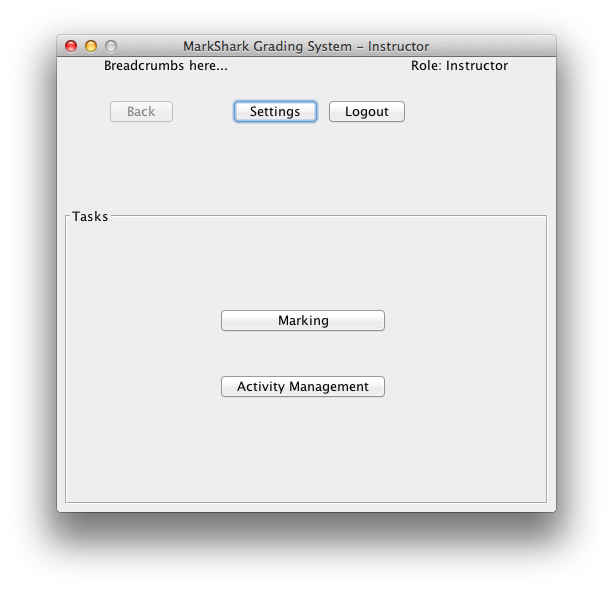
\includegraphics[scale=0.65]{../images/UpdatedUIScreens/landinginstructor.png}}
\label{landPg}
The Landing Page is shown to all users of the system following a successful login. The Tasks box will populate with the tasks available to the user, depending on their user type. For example, the preceding image shows the landing page of an Instructor.\\
\clearpage

\subsection{Manage Courses}
\begin{itemize}
	\item The user must log in to the system as an Administrative Assistant.
\end{itemize}
The following screen will be shown. Press the "Course Management" button.
   \begin{center}
     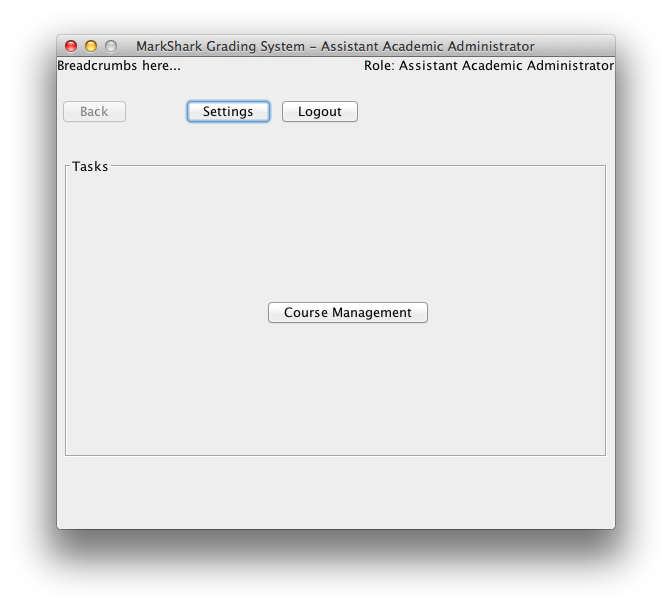
\includegraphics[scale=0.55]{../images/UpdatedUIScreens/landingassist.png}
   \end{center}
The "Course Management" Screen, shown above, will be displayed. On this screen, the user may  create a new course, or modify/delete an existing coruse.
\clearpage

\subsection{Create A Courses}
\begin{itemize}
	\item The user must log in to the system as an Administrative Assistant.
	\item The user has navigated to the "Create A Course" page.
\end{itemize}
The user will be presented with the following screen:
\begin{center} 
   	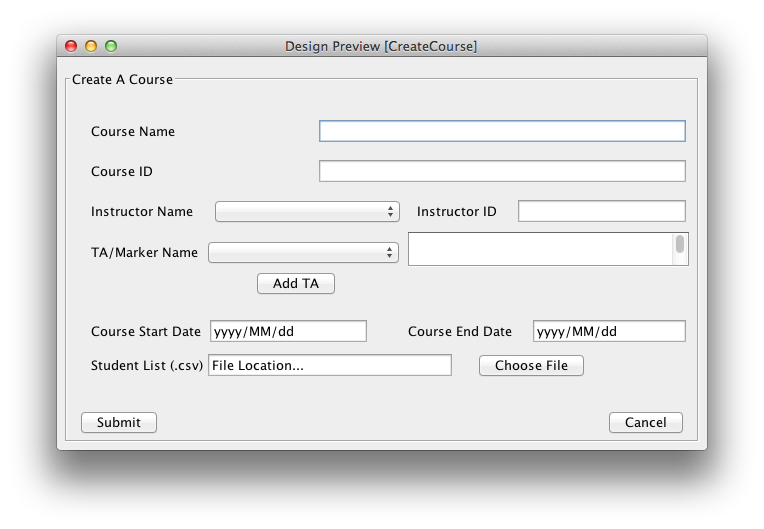
\includegraphics[scale=0.55]{../images/UpdatedUIScreens/CreateCourse.png}
\end{center} 
To create an activity, the user must enter values into the following fields:
\begin{itemize}
	\item Course Name/ID
	\item Instructor Name/ID
	\item Course Start/End Date
\end{itemize}
The user may also add TA marekers and a csv file of students (format: name, id)\\
\clearpage

\subsection{Modify A Course}
\begin{center} 
   	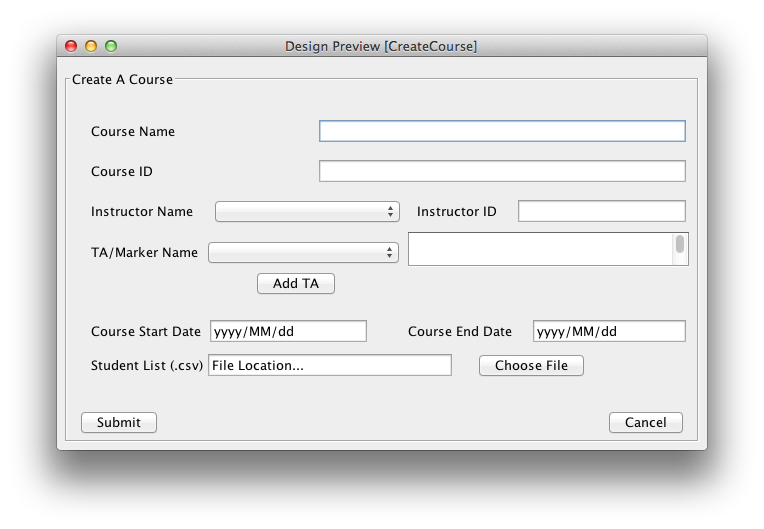
\includegraphics[scale=0.55]{../images/UpdatedUIScreens/CreateCourse.png}
\end{center} 
Rhe user may also use this page to modify any fields in the course, as well as add TAs and update the list of students.
\clearpage

\subsection{Create Activity (Detailed)}
\begin{enumerate}
  \item Log in to the system as an Instructor.
  \item The following screen will be shown.
    Press the \textbf{Assignment Management} button.
  \begin{center} 
   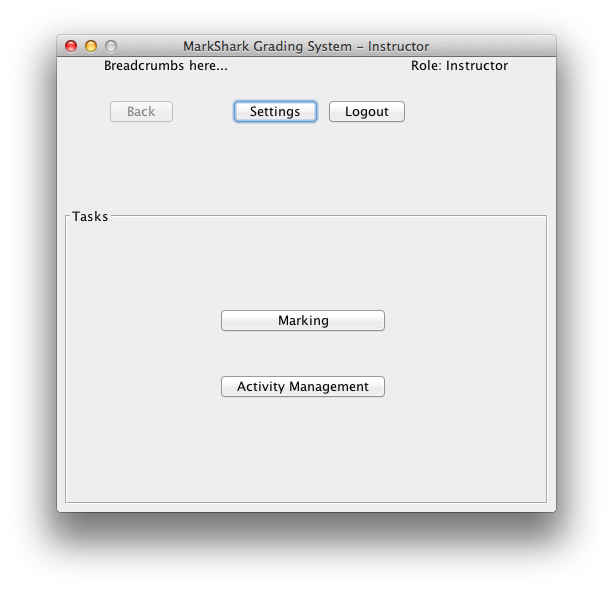
\includegraphics[scale=0.55]{../images/UpdatedUIScreens/landinginstructor.png}
  \end{center}
  \item The following screen will be shown.  Select the course that you wish
    to do make an activity for from the drop-down list, then press \textbf{Ok}.
    \begin{center} 
      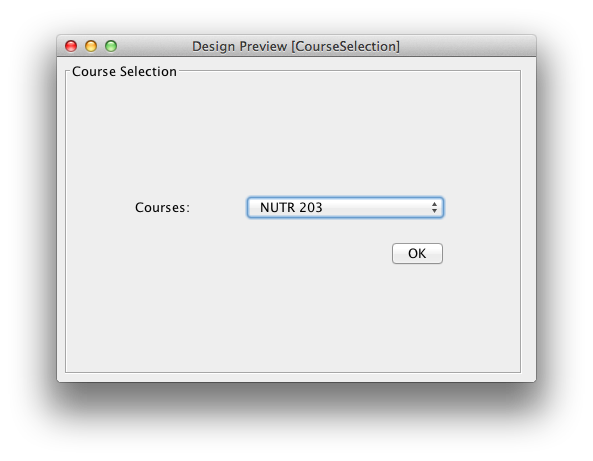
\includegraphics[scale=0.55]{../images/UpdatedUIScreens/CourseSelection.png}
    \end{center}
  \item The following screen will be shown.  Students are listed down the left
    side. Available activities are listed along the top.  Find the student you
    wish to mark for, and select the corresponding activity, then press \textbf{Ok}.
  \begin{center} 
     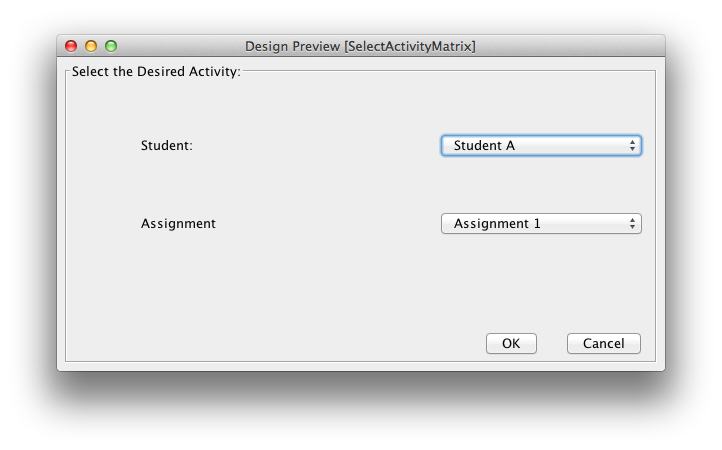
\includegraphics[scale=0.55]{../images/UpdatedUIScreens/MarkingActivitySelection.png}
  \end{center} 
  \item The following screen will be shown.
   \begin{center} 
   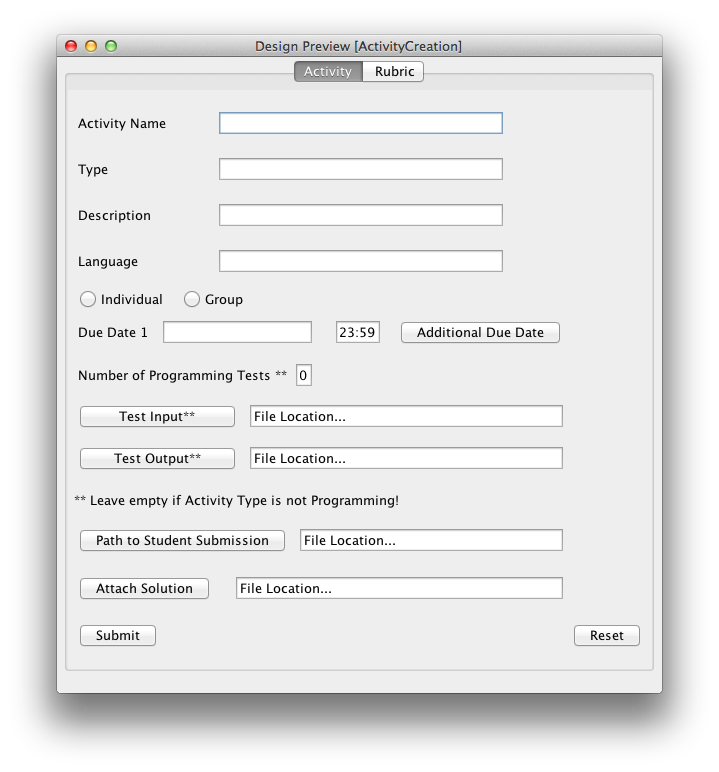
\includegraphics[scale=0.55]{../images/UpdatedUIScreens/ActivityCreation.png}
   \label{newActivity}
  \end{center}
  To create the activity, complete the following:
  \begin{enumerate}
  \item Enter a name for the activity in the \textbf{Name} text field by clicking on 
  it and typing it in.
  \item Select the type of the activity from the \textbf{Type} drop down box.
  This can be an Essay, a Problem Set, or a Programming activity.
  \item Enter a description for the activity by clicking on the \textbf{Description} 
  text field and typing it in.
  \item Enter the language of the activity by clicking on the \textbf{Language} text
  field and typing it in. This can be either a spoken language such as English 
  for an Essay or Problem Set, or a programming language such as Java for a Programming
  activity.
  \item Click on the appropriate radio to make it an \textbf{Individual} or 
  \textbf{Group} activity. If \textbf{Group} is chosen, type in the group size in the 
  adjacent field.
  \item Enter the date and time the activity is due in the \textbf{Due Date} fields 
  in the Year, Month, Day format, followed by the time it is due on that due in
  the 24-hour format. The default time is 23:59.
  \item A solution can be attached by clicking the \textbf{Attach Solution} button and 
  selecting the desired file from the Explorer window. Alternatively, the path can be 
  typed directly into the adjacent field.
  
  \item Clicking \textbf{Add Due Date} adds new fields to add an additional
    date that can be before or after the original due date. The new date can
    be entered in the same manner as as above. The extra field is the multiplier
    for penalties/bonuses. For example, entering "75" is equivalent to a 25\%
    penalty, and entering "110" would be equivalent to a 10\% bonus.
  \item The option \textbf{Attach Test Input/Output} becomes available if \textbf{Type} 
  is set to \textbf{Programming}. This functions exactly as \textbf{Attach Solution}.
 \end{enumerate}
 \item To work on the rubric for the activity, click on the \textbf{Rubric} tab at the 
 top of the page that is underneath the breadcrumbs. This will open the rubric tab and 
 show the following screen.
 \begin{center} 
	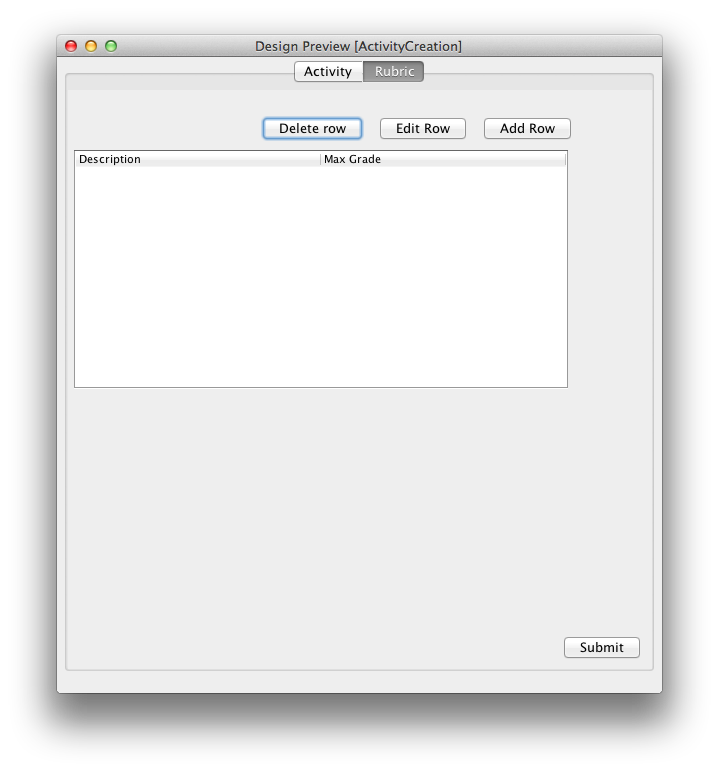
\includegraphics[scale=0.55]{../images/UpdatedUIScreens/RubricCreation.png}
 \end{center}
 \item Once all the desired information about the activity has been entered
   in correctly, clicking \textbf{Finish} will create the activity and open
   the \textbf{Activity Management} page.
\end{enumerate}
\clearpage

\subsection{Modify Activity}
Upon selecting \textbf{Modify Activity}, the activity selection screen will be shown.
  \begin{center} 
     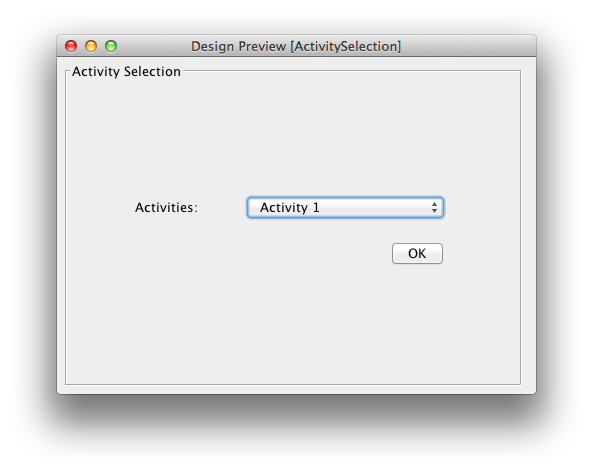
\includegraphics[scale=0.55]{../images/UpdatedUIScreens/ActivitySelection.png}
     \label{actSel}
  \end{center} 
  After selecting the activity, a screen will be shown that is the same as for 
  \textbf{New Activity} but with the fields already completed. Make edits as
  desired and complete in the same way as for \textbf{New Activity}.
\clearpage

\subsection{Activity Marking (Detailed)}
\begin{enumerate}
  \item Log in to the system as a user who has marking privileges.
  \item The following screen will be shown.  Press the \textbf{Marking} button.
  \begin{center} 
   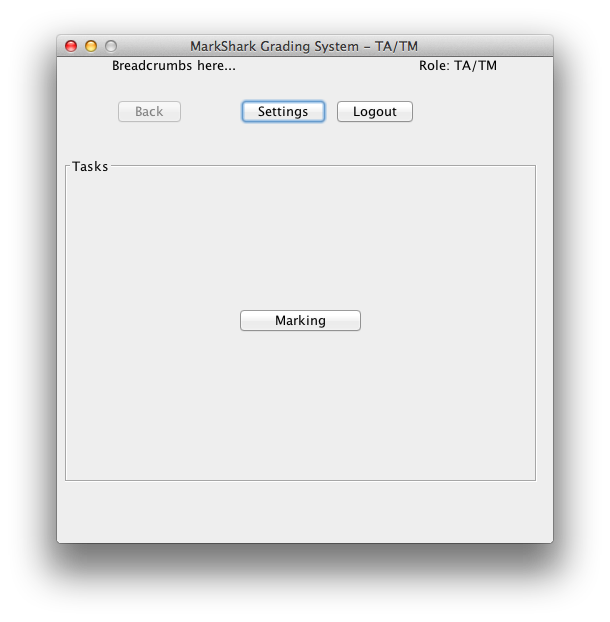
\includegraphics[scale=0.55]{../images/UpdatedUIScreens/landingTA.png}
  \end{center}
  \item The following screen will be shown.  Select the course that you wish
    to do marking for from the drop-down list, then press \textbf{Ok}.
    \begin{center} 
     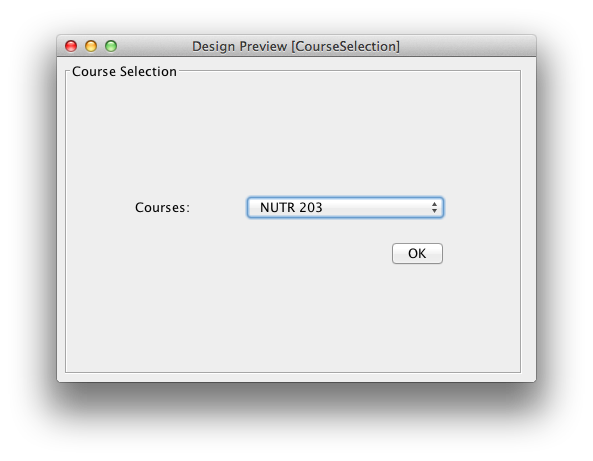
\includegraphics[scale=0.55]{../images/UpdatedUIScreens/CourseSelection.png}
     \label{courseSel}
    \end{center}
  \item The following screen will be shown.  Students are listed down the left
    side. Available activities are listed along the top.  Find the student you
    wish to mark for, and select the corresponding activity, then press \textbf{Ok}.
  \begin{center} 
    \includegraphics[scale=0.55]{../images/UpdatedUIScreens/mARKINGActivitySelection.png}
    \label{actSel}
  \end{center}
  \item The assignment's marking screen will be shown.  The marking screen
    displays the rubric, sample solution, and the student's submission. This is for a PDF assignment.
  \begin{center} 
   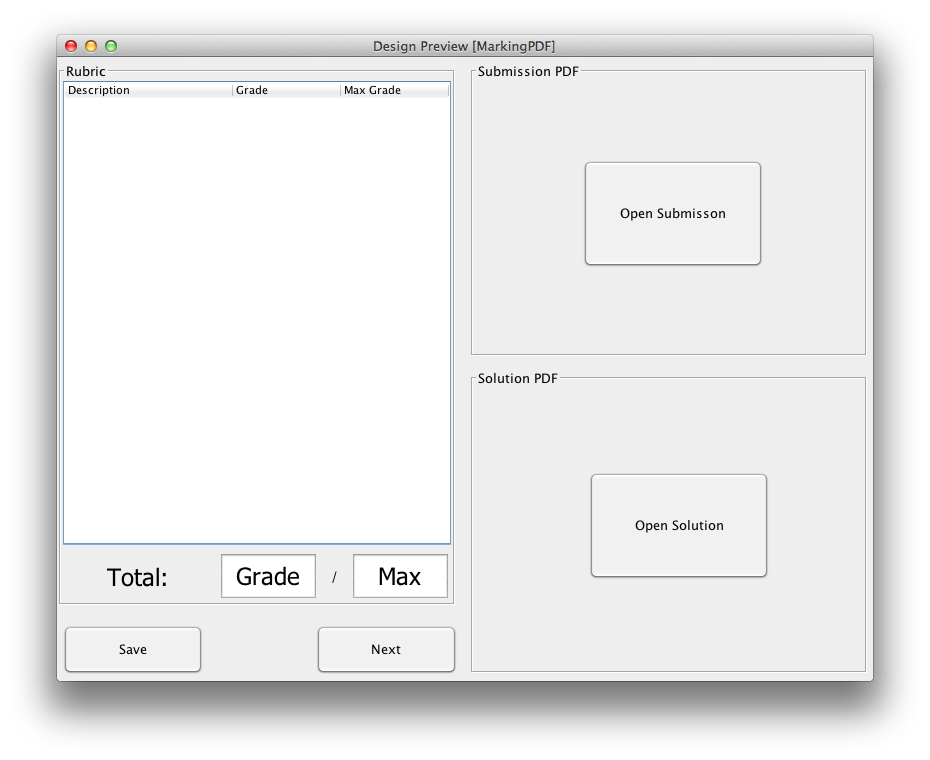
\includegraphics[scale=0.55]{../images/UpdatedUIScreens/MarkingPDF.png}
   \label{marking}
  \end{center}
    Perform the grading process as follows:
    \begin{enumerate}
      \item Perform necessary analysis on the student's work. 
      \item Read rubric points and enter a number into the available box 
        based on your analysis of the student's work.
      \item Repeat step (a) for remaining rubric points.
      \item A total will be shown at the bottom of the rubric to reflect the
        student's final grade on the activity.
       \item Click the \textbf{Submit} button to update the marks database with
         the changes made.
         \item If desired: Press the \textbf{Submit} button to move to the next
    student's submission of the same activity.
    \end{enumerate}
\end{enumerate}
\clearpage

\subsection{Student Code Testing}
\begin{center}
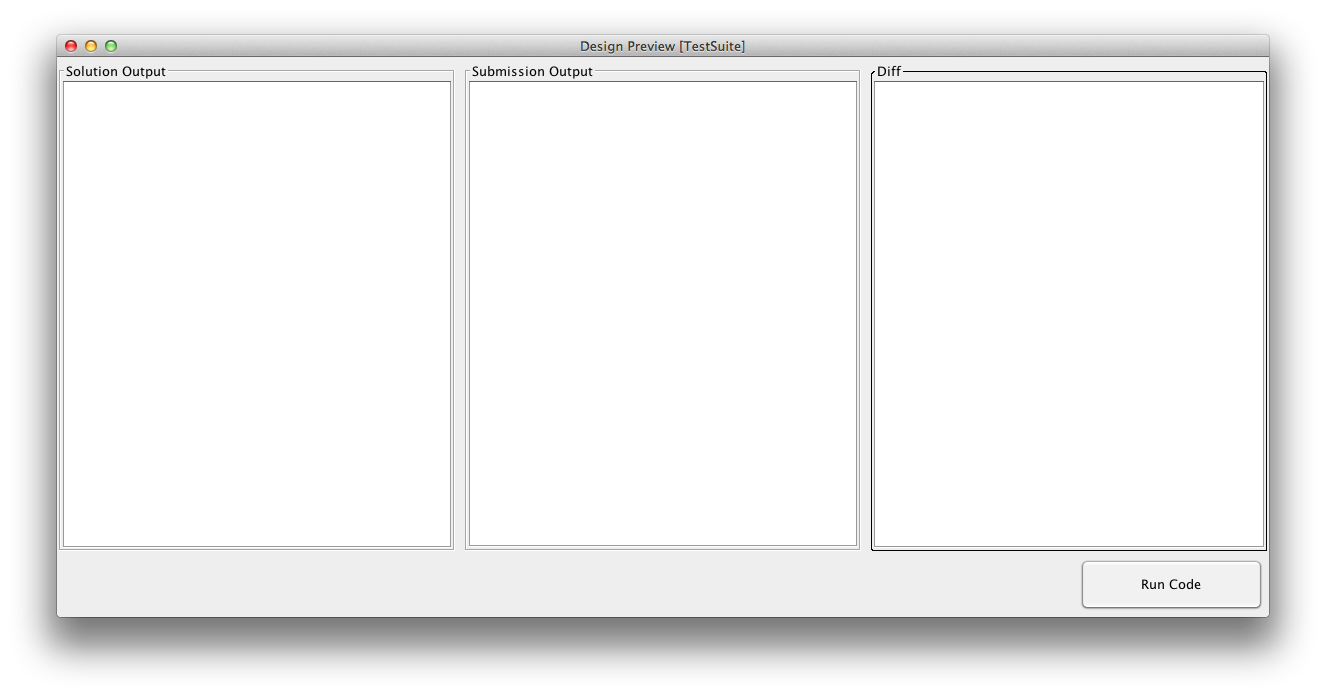
\includegraphics[scale=0.55]{../images/UpdatedUIScreens/TestSuite.png}
\label{testSuite}
\end{center}
The Test Suite shows the \textbf{Solution Output}, the \textbf{Student Output},
and the \textbf{Diff}.
The three windows can be docked together (tabbed) or positioned that each
window takes up $\frac{1}{3}$ of the screen space.
The \textbf{Diff} window intelligently shows the difference between
solution and submitted code.
\clearpage

\subsection{Manage User Accounts}
\centerline{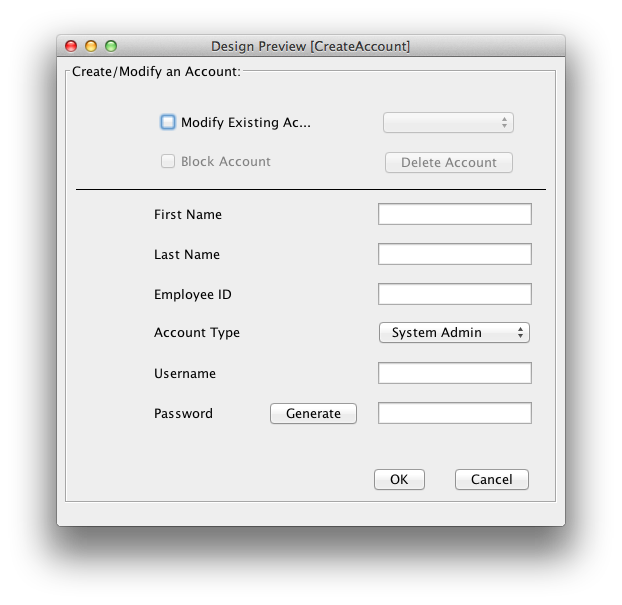
\includegraphics[scale=0.55]{../images/UpdatedUIScreens/CreateAccount.png}}
\label{manageAccts}
A form will appear on clicking this. 
If the user wishes to modify an existing account: \\
the user must check the \textbf{Modify} check-box. The grayed out drop down menu and
save button will become active, and the \textbf{Create} button will be grayed out.
The user will select the account to edit (organized alphabetically by username).
Upon selecting a user, the form fields will populate and become editable. After
the user has finished editing the fields, the user must click \textbf{Save}. The system
will save the changes and return to the Landing page. \\
\textbf{*NOTE*} If the user wishes to generate a new password, a confirmation
prompt will appear asking for confirmation.\\
If the user wishes to create a new account: \\
The user must not check the \textbf{Modify} box. By doing so, the \textbf{Save}
button and the drop-down menu for selecting an account will be grayed out.
The user then fills the form as normal. After the user has finished, the user
must click \textbf{Save}.
\clearpage

% ---
\section{Quick Reference}  % 9 Marks
\subsection{General Interface}
Each screen of the system (outside of the login screen) contains a unified top bar. \\
\centerline{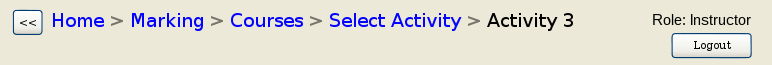
\includegraphics[scale=0.55]{../images/UIMockups/pngs/topBar}}
\begin{itemize}
  \item The leftmost $<<$ button causes the system to go back one screen. 
  \item Clicking on any of the links in the ``Breadcrumbs'' menu causes the system 
    to return to the screen related to that link. 
  \item The Logout button will work on any screen to log the user out and return
    them to the login screen.
  \item The \emph{Role} field will dynamically update with the role of the currently logged
    in user.
  \item Any time a user attempts to leave a screen where they have entered data or
    done some work, a confirmation will appear asking you whether you are sure
    you wish to navigate away from the page without saving it.
\end{itemize}

\subsection{System Administrator}
\centerline{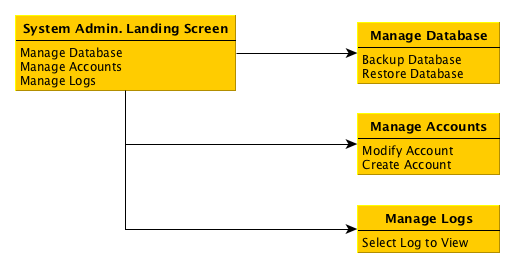
\includegraphics[scale=0.6]{../images/UIMockups/pngs/sysAdmin}}
\begin{itemize}
  \item To begin, log into the system through the login screen (page \pageref{login})
    by entering a valid username and password for a System Administrator account.
  \item Upon login, the \textbf{System Administrator Landing Page} (page 
    \pageref{landPg}) is displayed. The landing page contains Manage Database, 
    Manage User Accounts, and Manage System Logs buttons.
    \begin{itemize}
      \item If you select Manage Database, the \textbf{Manage Database screen} 
	(page \pageref{manageDB}) is displayed. This screen contains two 
	options, one for backing up the database and one for restoring it from 
	a previous backup. If you click on Backup Database then the database
	will be backed up to a specified location. If you click on Restore 
	Database, the system will prompt for a system backup, and restore
	the system based on it.
      \item If you select Manage User Accounts, the \textbf{User Account 
	Management screen} (page \pageref{manageAccts}) is displayed. If you are
	modifying an account, tick the Modify Account and select the account to
	modify, then update any details and save the changes. If you are creating an
	account, leave the modify box unticked, enter all details, and click save to
	create the account.
      \item If you select Manage System Logs the \textbf{System Log Management 
	screen} (page \pageref{manageLogs}) is displayed. This screen presents 
	you with a drop down menu from which you can select a log file for the 
	specified day of the system's usage, which will be displayed when selected.
    \end{itemize}
\end{itemize}

\subsection{Administrator}
\centerline{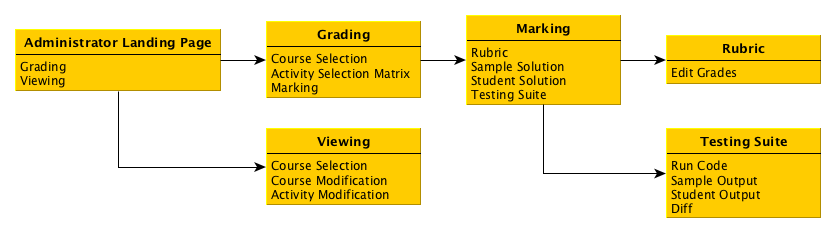
\includegraphics[scale=0.6]{../images/UIMockups/pngs/admin}}
\begin{itemize}
  \item To begin, log into the system through the login screen (page \pageref{login})
    by entering a valid username and password for an Administrator account.
  \item Upon login, the \textbf{Administrator Landing Page} (page \pageref{landPg})
    is displayed. The landing page contains two buttons: Grading and Viewing.
    \begin{itemize}
    \item If you select Grading, you will select a course from the complete list of 
      courses on the \textbf{Course Selection screen} (page \pageref{courseSel}). 
      You will then select an 
      activity to view or edit grades for, from all student from the \textbf{Activity 
    	 Selection Matrix screen} (page \pageref{actSel}). You can then view the 
	 grading of the specified
      activity and edit it as necessary on the \textbf{Marking screen} (page
      \pageref{marking}).
    \item If you select Viewing, you will be select a course from the complete list of 
      courses on the \textbf{Course Selection screen} (page \pageref{courseSel}). You can then view the
      details of that course on the \textbf{Course Modification screen} (page \pageref{createCourse})
      or view the details of any activities in it on the \textbf{Activity Modification screen}
      (page \pageref{newActivity}), but
      cannot edit any of the details of courses or activities.
    \end{itemize}
\end{itemize}

\subsection{Assistant Administrator}
\centerline{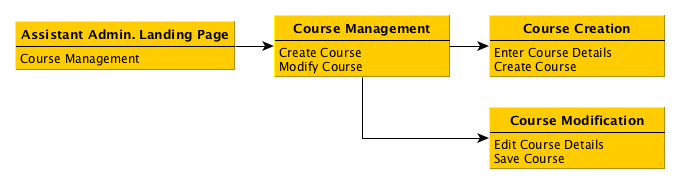
\includegraphics[scale=.6]{../images/UIMockups/pngs/assistantAdmin}}
\begin{itemize}
  \item To begin, log into the system through the login screen (page \pageref{login})
    by entering a valid username and password for an Assistant Administrator 
    account.
  \item Upon login, the \textbf{Assistant Administrator Landing Page} (page
    \pageref{landPg}) is displayed. There will be one button available: Course
    Management.
    \begin{itemize}
    \item When you select Course Management, the \textbf{Course Management
      screen} (page \pageref{courseManage}) will be displayed, with two buttons: 
      Create a Course and Modify a Course.
      \begin{itemize}
      \item If you select Create a Course, you will be sent to the \textbf{Course
	Creation screen} (page \pageref{createCourse}). Enter all the relevant details to creating a course, and
	confirm the course creation.
      \item If you select Modify a Course, you will be sent to the \textbf{Course
	Selection screen} (page \pageref{courseSel}) and will select a course from all the current courses
	available to be modified. After choosing a course, you are sent to the
	\textbf{Course Modification screen} (page \pageref{courseManage}). Change any relevant details about
	the course, and then confirm the course modification.
      \end{itemize}
    \end{itemize}
\end{itemize}

\subsection{Instructor}
\centerline{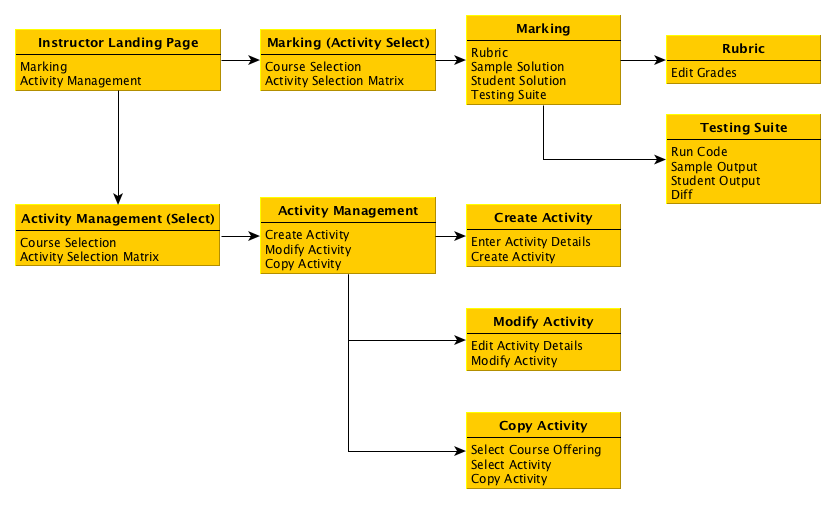
\includegraphics[scale=.6]{../images/UIMockups/pngs/instructor}}
\begin{itemize}
  \item To begin, log into the system through the login screen (page \pageref{login})
    by entering a valid username and password for an Instructor account.
  \item Upon login, the \textbf{Instructor Landing Page} (page \pageref{landPg}) 
    is displayed. There will be two buttons visible: Marking and Assignment 
    Management.
    \begin{itemize}
      \item If you select Marking, you will select a course from your list of courses
        on the \textbf{Course Selection screen} (page \pageref{courseSel}). You will then select an activity
        to mark for an available student from the \textbf{Activity Selection screen}
        (page \pageref{actSel}).
        \begin{itemize}
        \item You will then be sent to the \textbf{Marking screen}. (page
	  \pageref{marking}) You will enter grades into the rubric while viewing 
	  the student's submission side by side. If you click on the Sample Solution 
	  tab, the Rubric will be replaced with a sample solution to the assignment 
	  (the Rubric tab can then be reselected at any time). If you click Submit 
	  Grades the grades entered in the rubric will be saved, and you will 
	  move to the next student's submission. If you click Next, the you will 
	  move to the next student's submission, and a confirmation will be displayed 
	  asking if you are sure you want to navigate away if you have made any 
	  changes. If you click Submit Comments, any comments you have made 
	  on the student's work will be saved.
	  \begin{itemize}
	    \item If you click on Test Code, the \textbf{Test Suite} (page 
	      \pageref{testSuite}) screen is displayed. The test suite will allow you 
	      to run the student's code and compare its output with a sample 
	      solution's output. Clicking on the Diff tab will show a color coded 
	      comparison between the sample solution output and the student's 
	      output. Clicking on Run will run the student's code. Clicking on Stop 
	      will stop the code running (useful if it is stuck or hanging).
	  \end{itemize}
	\end{itemize}
      \item If you select Activity Management, you will then select a course from your
	list of courses on the \textbf{Course Selection screen} (page \pageref{courseSel}). The \textbf{Activity 
	  Management screen} is then displayed, with three buttons available: New 
	Activity, Modify Activity, and Copy Activity.
	\begin{itemize}
	\item If you select New Activity, the \textbf{New Activity screen} 
	  (page \pageref{newActivity}) is displayed.
	  Enter all relevant information to the assignment on this page. Clicking on
	  the Rubric tab will swap to a new tab for entering the details of the rubric.
	  You can navigate freely between the two tabs at any point. After entering
	  all fields, click on Finish and the activity will be created.
	\item If you select Modify Activity, the \textbf{Activity Selection screen} (page \pageref{actSel}) is
	  displayed. You will select an activity from the current course, and the
	  \textbf{Activity Modification screen} (page \pageref{newActivity}) 
	  will be displayed with all the current
	  info for the selected activity. You will update any desired info, along with
	  any of the details in the rubric. You can swap between the Rubric and 
	  Activity tabs at any time to edit details for the activity itself or
          the rubric.
	  After updating the activity, click Finish and any changes will be made.
	\item If you select Copy Activity, the \textbf{Copy Activity screen}
          is displayed.
	  You will see a list of previous course offerings along with all courses you
	  have previously taught. When you select one of these courses, you will
	  then see a list of activities available for copy. You can then select an
	  activity to copy, and after filling in an appropriate Due Date, add 
	  it to the course.
	\end{itemize}
    \end{itemize}
\end{itemize}

\subsection{Teaching Assistant}
\centerline{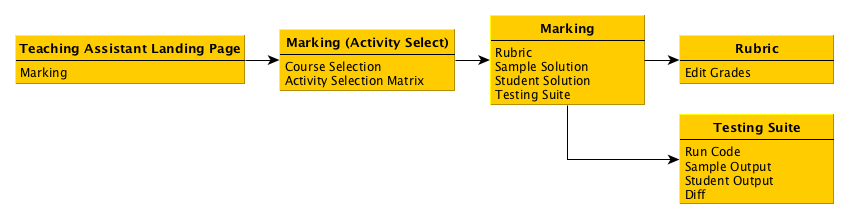
\includegraphics[scale=.6]{../images/UIMockups/pngs/teachingAsst}}
\begin{itemize}
  \item To begin, log into the system through the login screen (page \pageref{login})
    by entering a valid username and password for a Teaching Assistant account.
  \item Upon login, the \textbf{Teaching Assistant Landing Page} (page \pageref{landPg}) 
  	is displayed. The only button available on the landing page will be Marking.
    \begin{itemize}
      \item After clicking on Marking, you will select a course from your list of courses
	on the \textbf{Course Selection screen} (page \pageref{courseSel}). You will then select an activity
	to mark for an available student from the \textbf{Activity Selection Matrix
	  screen} (page \pageref{actSel}).
	\begin{itemize}
	  \item You will then be sent to the \textbf{Marking screen}. (page
	    \pageref{marking}) You will enter grades into the rubric while viewing 
	    the student's submission side by side. If you click on the Sample Solution 
	    tab, the Rubric will be replaced with a sample solution to the assignment 
	    (the Rubric tab can then be reselected at any time). If you click Submit 
	    Grades the grades entered in the rubric will be saved, and you will 
	    move to the next student's submission. If you click Next, the you will 
	    move to the next student's submission, and a confirmation will be displayed 
	    asking if you are sure you want to navigate away if you have made any 
	    changes. If you click Submit Comments, any comments you have made 
	    on the student's work will be saved.
	    \begin{itemize}
	      \item If you click on Test Code, the \textbf{Test Suite} (page 
		\pageref{testSuite}) screen is displayed. The test suite will allow you 
		to run the student's code and compare its output with a sample 
		solution's output. Clicking on the Diff tab will show a color coded 
		comparison between the sample solution output and the student's 
		output. Clicking on Run will run the student's code. Clicking on Stop 
		will stop the code running (useful if it is stuck or hanging).
	    \end{itemize}
	\end{itemize}
    \end{itemize}
\end{itemize}

% ---
\section{Known Bugs}
\section{Known Bugs}
\begin{itemize}
\item On pages with Submit buttons and corresponding information fields, if you click Back or Cancel, you will always be prompted that there might be changes that are unsaved.  This is only a bug in the case where the user has not made any changes.
\item Marking PDF screen gets cut off if the screen resolution is too small.
\item The shark on the Login Screen will be angry if you bother him.  (Click the Shark)
\item 
\end{itemize}

\end{document}
